
%% Template by Michal Forisek


\documentclass[12pt,a4paper]{report}
%\usepackage{slovak}
\usepackage[utf8]{inputenc}
\usepackage[IL2]{fontenc}
%\usepackage{a4wide}
\usepackage{tabularx}
\usepackage{amsfonts}
\usepackage{amssymb}
\usepackage{amsmath}
\usepackage{amsthm}
\usepackage{mathtools}
%\usepackage{breqn} % messes up biblatex and \log_2
%\usepackage{epsfig}
\usepackage{color}
\usepackage{mathrsfs}
\usepackage{verbatim}
\usepackage{fancyvrb}
\usepackage{float}
\usepackage{longtable}
\usepackage{listings}
\usepackage{graphicx}
\usepackage{changepage}
\usepackage{caption}
\usepackage{subcaption}
\usepackage{multirow}
\usepackage{paralist}
\usepackage{pdfpages}
\usepackage{tikz}
\usepackage{gnuplot-lua-tikz}
\usetikzlibrary{arrows,positioning,shapes}
\usepackage[style=alphabetic,maxbibnames=47,backend=biber]{biblatex}
% vim: set fdm=marker:
%% Original by Michal Forisek

%% zakladne definicie
\newcommand{\quoteme}[1]{\clqq#1\crqq}
\def\todo#1{[{\color{red} TODO:} {\bf  #1}]}
\def\fixme#1{[{\color{red} FIXME:} {\bf  #1}]}
\def\verify#1{\todo{verify: #1}}

\def\problem#1{\textsc{#1}}
\def\graphcol#1#2{\problem{GraphColoring(#1, #2)}}
\def\sgkh#1{\problem{$#1$-SGKH}}
\def\sguh#1{\problem{$#1$-SGUH}}

\def\phi{\varphi}
\def\xor{\oplus}
\def\concat{\|}
%\def\inr{\in_{R}}
\def\toa #1 {\overset{#1}{\rightarrow}}
\def\inr{\overset{\$}{\leftarrow}}
\def\assign{\leftarrow}
\def\send{\rightarrow}
\def\isomorph{\cong}
\def\nsd{NSD}
\def\union{\cup}
\newcommand{\unit}[1]{\ensuremath{\, \mathrm{#1}}}
\newcommand{\mset}[1]{\ensuremath{\mathbb{#1}}}
\newcommand{\Zn}[1]{\ensuremath{\mset{Z}_{#1}}}
\DeclareMathOperator{\dlog}{dlog}
\def\code#1{\lstinline@#1@}
\def\classname#1{{\tt #1}}

\def\compactlist{
  \setlength{\itemsep}{1pt}
  \setlength{\parskip}{0pt}
  \setlength{\parsep}{0pt}
}

%% Labely s predefinovanym asociovanym textom
\makeatletter
\def\textlabel#1#2{%
  \@bsphack\begingroup
  \protected@write\@auxout{}{\string\newlabel{#2}{{\@currentlabel}{\thepage}{#1}{\@currentHref}{}}}%
  \endgroup\@esphack
}%
\makeatother


%%% original od Misofa:
%% {{{

\catcode`\@=11

\def\R{\mset{R}}
\def\cent{{c\kern-0.3em|\kern0.1em}}
\def\N{\mset{N}}

\let\eps=\varepsilon

\def\relupdown#1#2#3{\mathrel{\mathop{#1}\limits^{#2}_{#3}} }

\let\then=\Rightarrow
\let\neht=\Leftarrow

\def\krok#1{\relupdown{\Longrightarrow}{}{#1}}
\def\thenrm{\relupdown{\Longrightarrow}{}{rm}}

\def\bicik{\upharpoonright}
\def\B{{\mathbf B}}
\def\kodTS#1{{\tt <}#1{\tt >}}

\newtheorem{definicia}{Definícia}[section]
\newtheorem{HLPpoznamka}{Poznámka}[section]
\newtheorem{HLPpriklad}{Príklad}[section]
\newtheorem{HLPcvicenie}[HLPpriklad]{Cvičenie}
\newtheorem{zadanie}{Úloha}[section]
\newenvironment{poznamka}{\begin{HLPpoznamka}\rm}{\end{HLPpoznamka}}
\newenvironment{priklad}{\begin{HLPpriklad}\rm}{\end{HLPpriklad}}
\newenvironment{cvicenie}{\begin{HLPcvicenie}\rm}{\end{HLPcvicenie}}
\newtheorem{veta}{Veta}[section]
\newtheorem{lema}[veta]{Lema}
\newtheorem{dosledok}[veta]{Dôsledok}
\newtheorem{teza}[veta]{Téza}
% \newtheorem{dokaz}{Dôkaz}[section]

\newtheorem{definition}{Definition}[chapter]
\newtheorem{theorem}[definition]{Theorem}
\newtheorem{lemma}[definition]{Lemma}
\newtheorem{corollary}[definition]{Corollary}
\newtheorem{observation}[definition]{Observation}

\long\def\odsadene#1{
\leftskip=\parindent
\parindent=0pt
\vskip-5pt

\parskip=5pt
#1
\parskip=0pt

\parindent=\leftskip
\leftskip=0pt

} % end \odsadene




%%%%%%%%%%% PROSTREDIE PRE PISANIE KOMENTAROV

%\newenvironment{komentar}{%
%\vskip\baselineskip
%\tabularx{0.95\textwidth}{|X|}
%\sl
%}
%{\endtabularx
%\vskip\baselineskip
%}

\newenvironment{komentar}{%
\vskip\baselineskip\noindent
\tabularx{\textwidth}{>{\hsize=.2\hsize}X>{\hsize=1.8\hsize}X}
\sl ~ & \sl
}
{\endtabularx
\vskip\baselineskip
}

%\newenvironment{komentar}{%
%\vskip\baselineskip
%\trivlist\vspace{-4pt}\raggedleft\item\relax\tabularx{0.9\textwidth}{X}\sl}
%{\endtabularx\vspace{-4pt}\endtrivlist
%\vskip\baselineskip
%}

\newenvironment{dokaz}{\trivlist
  \item[\hskip \labelsep{\bfseries Dôkaz.}]}{\endtrivlist}
  
%\newenvironment{dokaz}{%
%\vskip\baselineskip\noindent
%\tabularx{\textwidth}{||X||}
%\sl
%}
%{\endtabularx
%\vskip\baselineskip
%}

%%%%%%%%%%% PROSTREDIE PRE MOJE ITEMIZE 

\newenvironment{myitemize}{%
\begin{itemize}
\itemsep-3pt
}
{\end{itemize}
}

%%%%%%%%%%% MATICKE MAKRA

\font\tenrm=csr10

\def\eps{\varepsilon}
% \def\R{{\mathbb R}}
\def\lvec#1{\overrightarrow{#1}}
\def\uhol{{\measuredangle}}
\def\then{\Rightarrow}
% \def\lg{{\rm lg}}
\def\lg{\log_2}
%\def\div{\mathbin{\rm div}}
\def\div{{\rm div}}
\DeclarePairedDelimiter{\ceil}{\lceil}{\rceil}
\DeclarePairedDelimiter{\floor}{\lfloor}{\rfloor}
\DeclarePairedDelimiter{\paren}{(}{)}

%%%%%%%%%%% PDF

%\newif\ifpdf
%\ifx\pdfoutput\undefined
%  \pdffalse
%\else
%  \pdfoutput=1 \pdftrue
%\fi

%%%%%%%%%%% OBRAZKY 

\newcommand{\myincludegraphics}[2][]{\includegraphics[#1]{images/#2}}

%%%%%%%%%%% SLOVNICEK

\openout2=\jobname.slo

\newcommand{\definuj}[3][]{%
\def\tmpvoid{}\def\tmpfirst{#1}%
\ifx\tmpvoid\tmpfirst%
  {\sl #2}\label{definicia:#2}\write2{#2 & #3 & \pageref{definicia:#2} \cr}%
\else%
  {\sl #2}\label{definicia:#2}\write2{#1 & #3 & \pageref{definicia:#2} \cr}%
\fi}

\newcommand{\definujsilent}[2]{%
\label{definicia:#1}\write2{#1 & #2 & \pageref{definicia:#1} \cr}%
}

\newcommand\myglossary{
  \immediate\closeout2 
  %\if@twocolumn\@restonecoltrue\onecolumn\else\@restonecolfalse\fi
  \chapter{Slovníček pojmov}
  \begin{tabular}{|l|l|r|}
  \hline
  {\bfseries slovenský pojem} & {\bfseries anglický preklad} & {\bfseries str.} \\ 
  \hline
  \InputIfFileExists{\jobname.srs}{}{~ & ~ & ~ \\}
  \hline
  \end{tabular}
  %\if@restonecol\twocolumn\fi
}

%%%%%%%%%%% UVODZOVKY

\catcode`\"=13
\def "{\begingroup\clqq\def "{\endgroup\crqq}}
\def\dospecials{\do\ \do\\\do\{\do\}\do\$\do\&%
  \do\#\do\^\do\^^K\do\_\do\^^A\do\%\do\~\do\"}

%%%%%%%%%%% DANGER BENDS 

\font\manual=manfnt % font used for the METAFONT logo, etc.
\def\dbend{{\manual\char127}} % dangerous bend sign

\newlength{\bendwidth}   \settowidth{\bendwidth}{\dbend}    \newlength{\hangwidth}

\def\hangone{%
  \hangwidth=\bendwidth%
  \advance\hangwidth 5pt%
  \hangindent\hangwidth%
}
\def\hangtwo{%
  \hangwidth=\bendwidth%
  \multiply\hangwidth 2%
  \advance\hangwidth 6pt% 
  \hangindent\hangwidth%
}

\def\medbreak{\par\ifdim\lastskip<\medskipamount \removelastskip\penalty-100\medskip\fi}
\let\endgraf=\par

\def\d@nger{\medbreak\begingroup\clubpenalty=10000
%\def\d@nger{\begingroup\clubpenalty=10000
%  \def\par{\endgraf\endgroup\medbreak} \noindent\hangone\hangafter=-2
  \def\par{\endgraf\endgroup} \noindent\hangone\hangafter=-2
  \hbox to0pt{\hskip-\hangindent\dbend\hfill}}
\outer\def\danger{\d@nger}

\def\dd@nger{\medbreak\begingroup\clubpenalty=10000
%  \def\par{\endgraf\endgroup\medbreak} \noindent\hangtwo\hangafter=-2
  \def\par{\endgraf\endgroup} \noindent\hangtwo\hangafter=-2
  \hbox to0pt{\hskip-\hangindent\dbend\kern1pt\dbend\hfill}}
\outer\def\ddanger{\dd@nger}

\def\enddanger{\endgraf\endgroup} % omits the \medbreak
\def\enddangerhop{\endgraf\endgroup\medbreak}




\def\@nakedcite#1#2{{#1\if@tempswa , #2\fi}}
\DeclareRobustCommand\nakedcite{%
  \@ifnextchar [{\@tempswatrue\@nakedcitex}{\@tempswafalse\@nakedcitex[]}}
\def\@nakedcitex[#1]#2{%
  \let\@citea\@empty
  \@nakedcite{\@for\@citeb:=#2\do
    {\@citea\def\@citea{,\penalty\@m\ }%
     \edef\@citeb{\expandafter\@firstofone\@citeb\@empty}%
     \if@filesw\immediate\write\@auxout{\string\citation{\@citeb}}\fi
     \@ifundefined{b@\@citeb}{\mbox{\reset@font\bfseries ?}%
       \G@refundefinedtrue
       \@latex@warning
         {Citation `\@citeb' on page \thepage \space undefined}}%
       {\hbox{\csname b@\@citeb\endcsname}} }}{#1}}

\long\def\FIXME#1{
  \begin{center}
  \begin{minipage}{0.8\textwidth}
  {\bf FIXME:~}\sl #1
  \end{minipage}
  \end{center}
}


\catcode`\@=12
%% }}}


\def\author{Michal Petrucha}
\def\supervisor{RNDr. Michal Forišek, PhD.}
\def\titlea{Selected Topics}
\def\titleb{from Advice Complexity}
\def\title{\titlea{} \titleb}
\def\thesistype{Diploma thesis}
\def\year{2014}
\def\location{Bratislava}
\def\department{Department of Computer Science}
\def\studyprogram{Informatics}
\def\fieldnumber{2508}
\def\university{Comenius University in Bratislava}
\def\faculty{Faculty of Mathematics, Physics and Informatics}

\usepackage[hidelinks]{hyperref}

\addbibresource{literature.bib}

\newlength{\firstpagewidthinc}
% The length by which we want the first two pages wider:
\setlength{\firstpagewidthinc}{2cm}
\graphicspath{{img/}}
\linespread{1.4}

\lstset{numberstyle=none, basicstyle=\ttfamily,
showstringspaces=false, escapechar=\%, language=C++}

% TODO: Move the setup of packages into a separate file.

% Set up hyperref...
\hypersetup{
    pdfauthor = {\author},
    pdftitle = {\titlea{} \titleb},
    pdfkeywords = {online problem} {advice complexity} {approximation}
}

\begin{document}

\newlength{\firstpagewidth}
\setlength{\firstpagewidth}{\textwidth}
\addtolength{\firstpagewidth}{\firstpagewidthinc}

\pagenumbering{roman}

%%%%%%%%%%%%%%%%%% Obal %%%%%%%%%%%%%%%%%%
\thispagestyle{empty}
% Tu je kopa zakomentovanych riadkov, lebo Pastorovej sa z nejakeho dovodu
% nepaci v niektorych pracach, ze maju na obale logo, zatial co pri inych
% jej to vobec nevadi, tak nech je spokojna.
\begin{adjustwidth}{-0.5\firstpagewidthinc}{-0.5\firstpagewidthinc}
%\begin{minipage}{0.25\firstpagewidth}
%
\includegraphics[width=0.9\textwidth]{img/komlogo-new}
%\end{minipage}
%\begin{minipage}{0.69\firstpagewidth}
\begin{center}
\textsc{\university} \\
\textsc{\faculty} \\
\end{center}
%\end{minipage}

\bigskip
%3dc8ac68-0ab2-4817-b352-48b4038e9b46

\vfill
\begin{center}
\begin{minipage}{0.8\textwidth}
%\hrule
\bigskip\medskip
\centerline{\LARGE\sc\titlea}
\smallskip
\centerline{\LARGE\sc\titleb}
\smallskip
\centerline{\thesistype}
\end{minipage}
\end{center}
\vfill
\vfill
{\bf\year}
\hfill{\bf\author}
\end{adjustwidth}
\eject % EOP i


%%%%%%%%%%%%%%%%%% Titulna strana %%%%%%%%%%%%%%%%%%
\thispagestyle{empty}
\begin{adjustwidth}{-0.5\firstpagewidthinc}{-0.5\firstpagewidthinc}
\begin{minipage}{0.25\firstpagewidth}

\includegraphics[width=0.9\textwidth]{img/komlogo-new}
\end{minipage}
\begin{minipage}{0.69\firstpagewidth}
\begin{center}
\textsc{\university} \\
\textsc{\faculty} \\
\end{center}
\end{minipage}

\vfill
\begin{center}
\begin{minipage}{0.8\textwidth}
%\hrule
\bigskip\medskip
\centerline{\LARGE\sc\titlea}
\smallskip
\centerline{\LARGE\sc\titleb}
\smallskip
\centerline{\thesistype}
\bigskip
\bigskip
%\centerline{\large\sc \author}
\bigskip\bigskip
%\hrule
\end{minipage}
\end{center}
\vfill
\begin{tabular}{l l}
Study programme: & \studyprogram \\
Field of study: & \fieldnumber{} \studyprogram \\
Department: & \department \\
Supervisor: & \supervisor \\
\end{tabular}
\vfill
{\bf\location, \year}
\hfill{\bf\author}
\end{adjustwidth}

\eject % EOP i

%%%%%%%%%%%%%%%%%% Zadanie %%%%%%%%%%%%%%%%%%
%\thispagestyle{empty}

%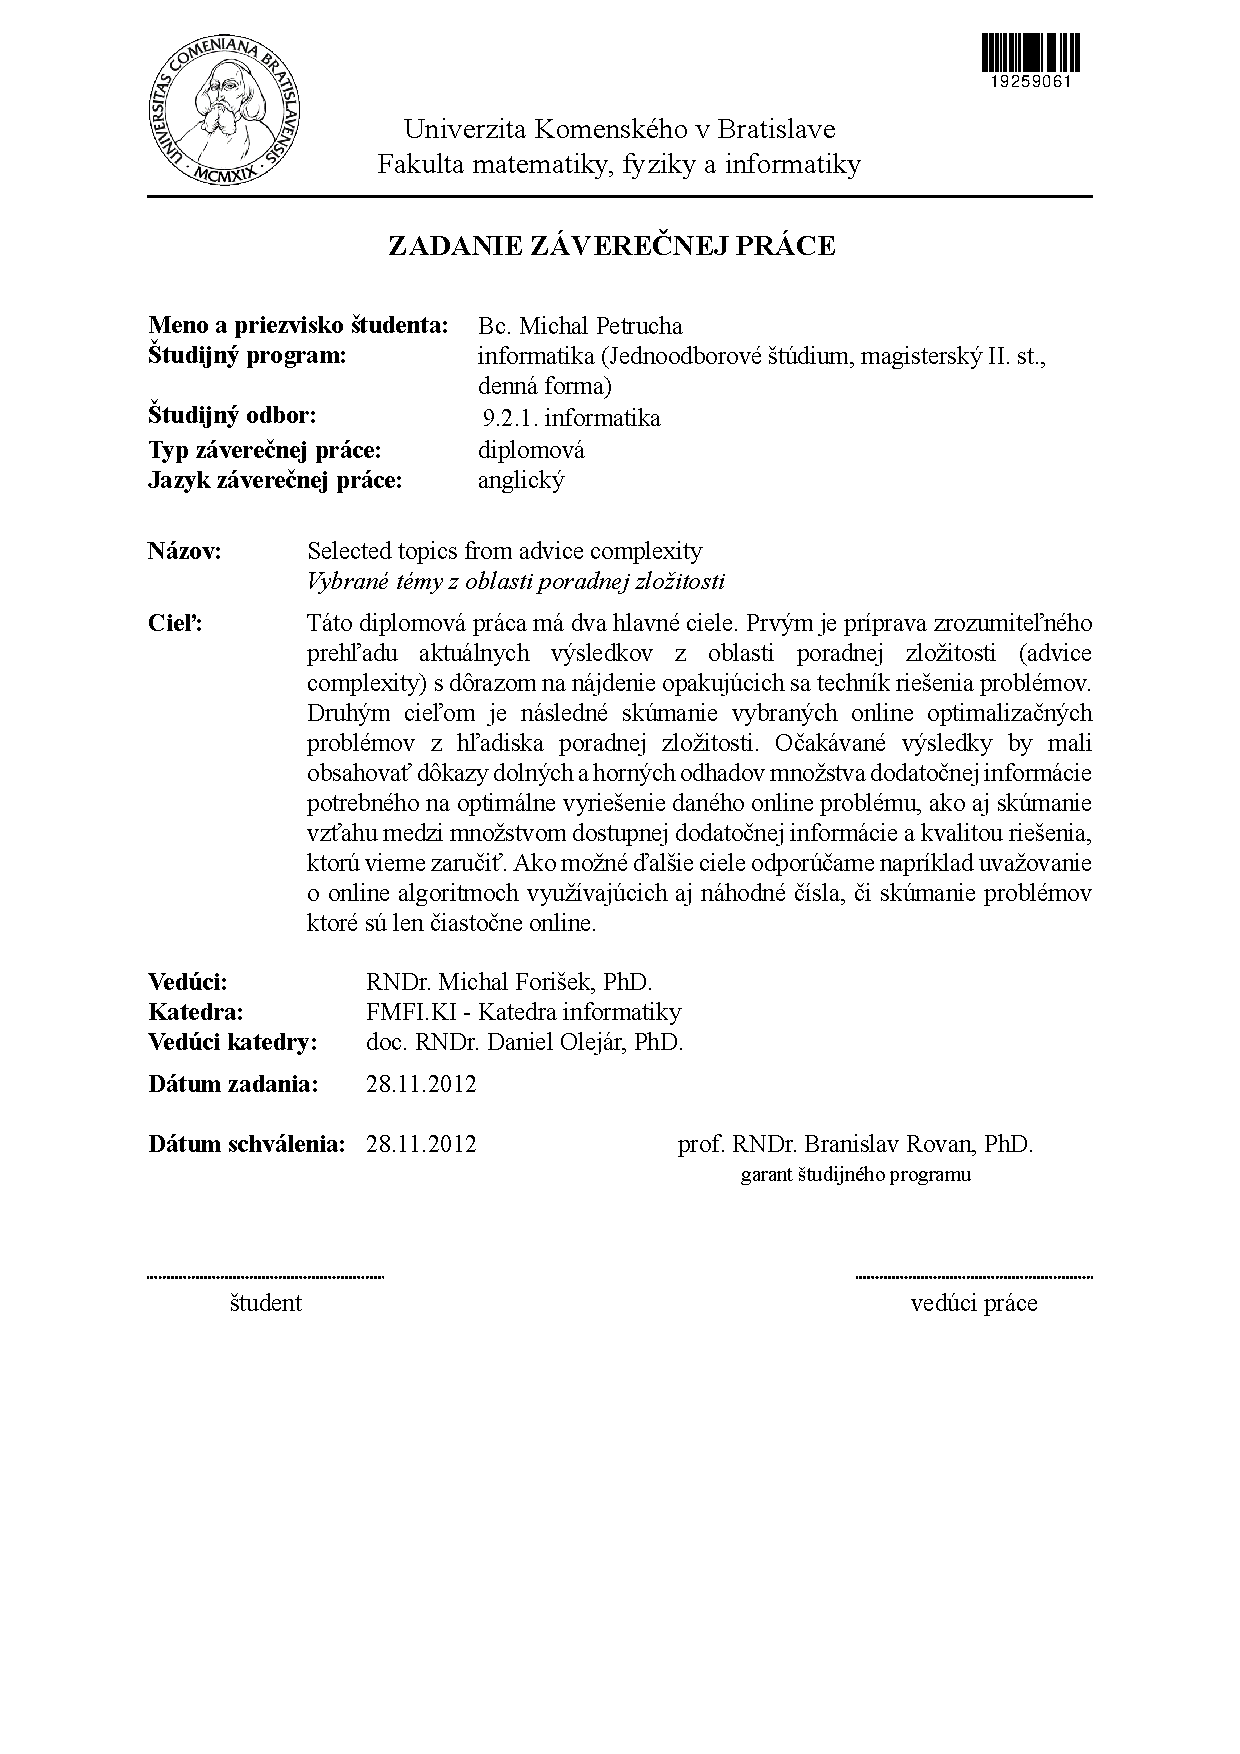
\includepdf{img/zadanie.pdf}

\eject

%\includepdf{img/statement.pdf}

\eject

%%%%%%%%%%%%%%%%%% Abstrakty a poďakovanie %%%%%%%%%%%%%%%%%%
%\thispagestyle{empty}
\section*{Abstrakt}
Sem patrí abstrakt v~slovenčine.

\medskip
{\bf Kľúčové slová:} nejaké sem treba doplniť



\eject

%\thispagestyle{empty}
\section*{Abstract}
This is where the abstract in English will go.

\medskip
{\bf Key words:} and some key words as well



\eject

\section*{Acknowledgements}
I want to thank Valve for their Holiday sales on Steam which gave me a lot
of options to procrastinate instead of working on this thesis.


\eject

%\thispagestyle{empty}
\tableofcontents
%\thispagestyle{empty}

% S tymito dvomi sa este bude treba pohrat, hlavne aby nemali cislovane
% strany a vobec.
\listoffigures
\listoftables

\chapter*{Introduction}
\pagenumbering{arabic}
\setcounter{page}{1}
\addcontentsline{toc}{chapter}{Introduction}
\label{chapter:intro}
This is the place for an introduction\dots


\chapter{First chapter}
\todo{Name this chapter!}
\label{chapter:first}

\todo{Write this introduction}
This is the sectionless introduction to the first chapter. Probably a word
or two about how we are going to give a brief overview of what online
problems and advice complexity are and the appropriate definitions upon
which this thesis is based.

\section{Online problems}
\label{section:online}
One of the countless ways to categorize algorithmic problems is into
\emph{offline} and \emph{online problems}. Offline problems are those
where the algorithm can access the whole input instance before yielding
the output.  On the other hand, the instance of an online problem is
revealed to the algorithm in smaller pieces and after each piece a partial
solution has to be produced. This partial solution cannot be changed
later.

A slightly different way of looking at online algorithms is that the
algorithm waits for an input query, processes it and outputs an answer to
this query immediately. Then it waits for another query and repeats the
process until there is nothing more to do.

Solving a problem online is obviously more difficult than solving the same
instance knowing the whole input at once. For many problems it is even
impossible to compute the optimal partial solutions without the knowledge
of the rest of the input sequence. Therefore we define a \emph{competitive
ratio} of an algorithm, which is the quotient of the cost of the solution
produced by the online algorithm and the cost of the optimal solution. An
optimal solution is one produced by an optimal offline algorithm. Since
the competitive ratio can depend on the input instance, we study the
worst-case competitive ratio an algorithm achieves.

We may consider randomized online algorithms as well. In this case we
examine the expected competitive ratio.

Let us describe a few examples of simple online problems to give a better
idea of what they are about. A very simple online problem is ski rental.
Suppose we are going to take an unknown number of ski trips and we do not
own a pair of skis. Renting a pair of skis for a single trip costs $1$,
buying one costs $s$. The input consists of a sequence of queries ``take a
ski trip'' and after each query an answer is expected that is either
``rent'', ``buy'' or ``use skis already bought''. In \cite{skirental} it
is proved that to minimize the competitive ratio the algorithm needs to
rent for the first $s-1$ rounds and then buy a pair of skis; this way, the
competitive ratio is $\frac{2s-1}{s} \approx 2$.

Another classic online problem is the paging problem. Assume a two-level
memory divided into uniform, fixed-size pages. Let $k$ be the number of
pages that can fit within the fast memory. The input consists of $n$
queries, each specifying a page we want to access. This page needs to be
loaded into the fast memory, thus replacing a page called a victim (unless
it is there already). The goal is to minimize the number of page faults,
i.e. the number of times we need to load a page from the slow memory into
the fast level.

In \cite{paging-deterministic} the authors show that for any deterministic
online algorithm solving the paging problem it is possible to construct an
instance using $k + 1$ pages where the online algorithm will produce a
page fault on each request by always choosing the page that is not in the
fast memory. However, an offline algorithm can decrease the number of page
faults by at least a factor of $k$, therefore the competitive ratio of any
online paging algorithm is at least $k$.

In addition, in \cite{paging-randomized} the authors describe a randomized
online algorithm for the paging problem whose competitive ratio is $H_k$.

\section{Advice complexity}
\label{section:advice}
In the previous section we showed that there are problems which cannot be
solved optimally by a deterministic online algorithm. This means that
having access to the whole of the input sequence can help the algorithm to
provide better partial results. However, sometimes it may not be necessary
to access the whole input sequence in order to compute the optimal
solution, in some cases a significantly smaller amount of information is
required.

That is why a computational model of \emph{online algorithms with advice}
has been introduced in \cite{advice-first}. In this model, the online
algorithm is assisted by an oracle with access to the entire input
sequence. The oracle has unlimited computational power and provides the
online algorithm with information about the input sequence that it
requires. We define the \emph{advice complexity} of an online algorithm as
the minimal number of bits it needs to read from the oracle in order to
solve the problem optimally. The advice complexity of an online problem is
then defined as the lowest advice complexity of online algorithms solving
it.

There have been multiple formal definitions of this model with various
drawbacks. \cite{advice-first} contains a definition in which the online
algorithm has access to a finite binary advice tape. That means, however,
that additional information can be encoded into the length of the advice
tape. In \cite{advice-constant} the authors define a slightly different
model where the online algorithm receives the same amount of information
in each round. This makes it impossible to use a sublinear amount of
advice. The model used in this thesis has been defined in
\cite{advice-infinite}; this model uses an infinite advice tape and we
measure the number of bits the algorithm accesses.

To illustrate the power of advice, we show the amount of advice required
to solve the two aforementioned online problems optimally. The ski rental
problem is trivial to solve using a single bit of advice -- this bit tells
the algorithm whether there will be at least $s$ queries. The online
algorithm reads this before answering the first query and it knows
immediately whether to buy a pair of skis or just rent them on each trip.

The paging problem is slightly more complex to solve optimally using
advice. Following the proof in \cite{paging-optimal}, this can be done
using $n$ bits of advice. The oracle calculates one optimal solution to
the input instance and assigns a single bit to each request. This bit
indicates whether the page will be accessed again before it is replaced by
another one in the optimal solution, such pages are called active; if the
page will not be accessed again, it is passive. The online algorithm then
just picks a passive page as the victim on each page fault.

Thus far we only covered the amount of advice required to obtain the
optimal solution using an online algorithm. However, it is also useful to
examine the amount of advice required to achieve a certain competitive
ratio and the tradeoff between these two. In this thesis we will study
this aspect as well.

Another possible area of research is the amount of advice required to
solve a \emph{partially online problem}. This is a special case of an
online problem where only a part of the input instance is served in pieces
and at some point the whole rest of the input is served in a single piece.

Taking the previous notion one step further, it also makes sense to apply
the concept of advice to offline problems. In that case, we no longer
study the competitive ratio. Instead, we can use advice to help an
algorithm achieve better efficiency, mainly in terms of its time
complexity, especially for known hard problems, such as $NP$-complete
problems. This direction of research is explored further in the last
chapter of this thesis.

\section{Online graph coloring}
\label{section:online-graph}
The main focus of this thesis is on the problem of online graph coloring.
Obviously, the difficulty of this problem depends greatly on any
assumptions we make on the input instance, e.g. restrictions on the class
of graphs, e.g. trees, bipartite graphs, cycles or a relationship between
the number of vertices and the number of edges, or the order in which
their vertices are revealed to the online algorithm. All these assumptions
provide the algorithm with additional information. This means that by
comparing the advice required to solve these special cases to the advice
complexity of the general case we can quantify the amount of information
provided by a particular set of assumptions.

An online graph coloring algorithm works roughly as follows. In each turn
a single vertex of the input graph is revealed to the algorithm and it has
to assign a color to this vertex. More precisely, assuming the vertices of
a graph are ordered in a sequence, in $t$-th turn the algorithm has the
knowledge of the subgraph induced by the first $t$ vertices in this
sequence. That means, all edges are revealed as soon as both of their
ending vertices are known.

The order in which vertices are revealed is referred to as the
\emph{presentation order}. In the most general case, the vertices will
appear in a fully arbitrary order. We can restrict this to a connected
presentation order, which means that in each turn the vertex currently
revealed is connected to at least one vertex revealed previously. This can
be restricted even further to the order in which a depth-first search
(\problem{DFS}) or a breadth-first search (\problem{BFS}) will visit
vertices. Another common presentation order is when the sequence of
vertices is sorted by their degrees.

In this thesis, each time we study a particular online graph coloring
problem, we specify explicitly both the class of graphs and the
presentation order. For instance, \graphcol{bipartite}{connected} denotes
that the problem is restricted to bipartite graphs and their vertices are
revealed in a connected order. As a special case, \graphcol{any}{any}
denotes the most general version of the problem where no assumptions are
made at all.

\section{Formal definitions and notations}
\label{section:definitions}
Having described the basic concepts in informal terms, let us now proceed
to formally define the model we are working with.

\begin{definition}[Online Algorithm]\label{def:online-algorithm}
    Let $I = (x_1, \dots, x_n)$ be an input sequence of an online problem.
    An \emph{online algorithm} $A$ computes the output sequence $A(I) =
    (y_1, \dots, y_n)$ such that $y_i = f(x_1, \dots, x_i)$ for some
    function $f$. We denote the cost of the solution computed by $A$ as
    $C(A(I))$.
\end{definition}

An optimal solution for $I$ will be denoted by $Opt(I)$. By optimal
solution we mean one which can be computed by an offline algorithm with
unbounded computational power, such that, in the case of maximization
problems, it maximizes the cost. We will use $E[X]$ to denote the expected
value of a random variable $X$.

\begin{definition}[Competitive Ratio]\label{def:competitive-ratio}
    Consider an optimization problem in which the goal is to maximize the
    cost of a solution. An algorithm $A$ is $c$-competitive if there is a
    constant $\alpha$ such that for each instance $I$ we have $C(A(I))
    \geq C(Opt(I)) / c - \alpha$. If $\alpha = 0$, we say that $A$ is
    strictly $c$-competitive. The \emph{competitive ratio} of $A$ is the
    smallest $c$ such that $A$ is $c$-competitive.
\end{definition}

For minimization problems, competitiveness is defined analogously, only
the inequality changes to $C(A(I)) \leq c \cdot C(Opt(I)) + \alpha$.

The previous definition can easily be extended to randomized algorithms.
For each instance $I$ we require $E[C(A(I))] \geq C(Opt(I)) / c -
\alpha$. We say that the expected competitive ratio of $A$ is the smallest
value of $c$ satisfying the above inequality.

We shall now extend the above definitions to include advice.

\begin{definition}[Online Algorithm with Advice]\label{def:online-advice}
    Consider an input sequence $I = (x_1, \dots, x_n)$ and an infinite
    binary string $\phi$.  An \emph{online algorithm $A$ with advice}
    computes the sequence $A^\phi(I) = (y_1, \dots, y_n)$ if $y_i =
    f(\phi, x_1, \dots, x_i)$. We call $\phi$ the \emph{advice string}.
\end{definition}

As stated earlier, the computation of $A$ can be interpreted as a series
of turns, where in the $i$-th turn the algorithm reads $x_i$ and yields
$y_i$ using all the information read so far and possibly some additional
bits from the advice string $\phi$. It is worth noting that the definition
does not restrict the computational power of $A$.

\begin{definition}[Advice Complexity]\label{def:advice-complexity}
    The \emph{advice complexity} of an algorithm $A$ is a function $s$
    such that $s(n)$ is the smallest value such that for each input
    sequence of size $n$ there is an advice string $\phi$ such that the
    algorithm $A$ examines at most the first $s(n)$ bits of $\phi$. The
    advice complexity of an online problem is the smallest advice
    complexity of an online algorithm which computes an optimal solution
    for each instance.
\end{definition}

\begin{definition}\label{def:advice-competitive}
    An online algorithm with advice $A$ is $c$-competitive if there is a
    constant $\alpha$ such that for every $n \in \N$ and for every
    instance $I$ of size at most $n$ there is an advice string $\phi$ for
    which $C(A^\phi(I)) \geq C(Opt(I)) / c - \alpha$ holds.
\end{definition}


\chapter{Known results and related work}
\label{chapter:known}
\todo{Write this chapter introduction}

In this chapter we give an overview of currently known results and
advances in the field of advice complexity.

\section{Common analysis and proof techniques}
\label{section:techniques}
\todo{Categorize this section into subsections: common prefix, partition
tree, anything else\dots?}

Despite the fact that the computational model of online algorithms with
advice has been only concieved a few years ago it is already possible to
notice the emergence of common techniques to analyze online problems and
find lower and upper bounds for their advice complexity.

To find an upper bound the most straightforward method is, same as with
other complexity metrics, to find an algorithm which solves the problem
and then determine its advice complexity. Any optimal algorithm cannot
then have any worse advice complexity. While this method is obvious, it is
often the most demonstrative one.

Proving lower bounds is usually significantly more difficult. Instead of
showing an algorithm which does not need more than a certain amount of
advice, to prove that $b$ is a lower bound, we need to show that any
algorithm with a certain guarantee on the competitive ratio cannot achieve
this without reading at least $b$ bits.

\subsection{Common prefix}

Probably the most basic approach to find the lower bound on the advice
complexity of a particular online problem is to find a set of instances
with the following properties:

\begin{enumerate}[(i)]
    \item
    for a given non-negative integer $k$ the prefixes $(x_1^{(i)}, \dots,
    x_k^{(i)})$ of instances $I^{(i)}$ are equal, i.e., for two instances
    $I^{(i)} \not= I^{(j)}$, for each $l$ such that $1 \leq l \leq k$,
    the members $x_l^{(i)}$ and $x_l^{(j)}$ are equal

    \item
    for each pair of instances $I^{(i)} \not= T^{(j)}$ there are no
    optimal solutions $Opt(I^{(i)}) = (y_1^{(i)}, \dots, y_{n_i}^{(i)})$,
    $Opt(I^{(j)}) = (y_1^{(j)}, \dots, y_{n_j}^{(j)})$ such that
    $$
        (y_1^{(i)}, \dots, y_{k}^{(i)}) = (y_1^{(j)}, \dots, y_{k}^{(j)})
    $$
\end{enumerate}

In other words, we find a set of instances such that the algorithm cannot
possibly distinguish the prefixes of these instances, however, for each
instance a unique solution needs to be yielded in the prefix already. To
achieve this, the advice string must necessarily be used. If the size of
this set of instances is $m$, at least $\lg m$ advice bits need to be
accessed which gives a lower bound on the advice complexity of the
problem.

This technique is used in various proofs in \cite{misof-trivial-graphs}
and in \cite{komm-thesis} to prove a lower bound on the advice complexity
of disjoint path allocation.

It is possible to generalize this technique to show lower bounds not only
on the advice complexity of an optimal solution, but also to show lower
bounds for $c$-competitive algorithms for a given constant $c$.

In this case, it is useful to look at an online algorithm with $b$ bits of
advice as a collection of $2^b$ deterministic online algorithms with
different strategies. If the problem in question has the property that a
strategy (sequence of decisions on the common prefix) leading to an
optimal solution for a particular instance $I$ also leads to a competitive
solution for a set of similar instances, we can estimate an upper bound on
the number of such similar instances, let us denote this by $s$. A lower
bound on the number of required strategies is then obtained as $m/c$,
which means that $\log\frac{m}{b}$ is a lower bound on the number of
advice bits.

\subsection{Reduction to string guessing}

In \cite{string-guessing} the authors use reductions to a simpler problem
that is easier to analyze as a method to prove lower bounds. Specifically,
they picked the string guessing problem in two variants.

\begin{definition}[String Guessing with Known History]
    The string guessing problem with known history over an alphabet
    $\Sigma$ of size $q \geq 2$ (denoted as \sgkh{q}) is defined as
    follows. The input instance $I = (n, d_1, \dots, d_n)$ consists of an
    integer $n$ specifying the length of the instance and a sequence of
    $n$ characters, where $d_i \in \Sigma, 1 \leq i \leq n$. Let $A$ be an
    online algorithm that solves \sgkh{q}, then $A(I) = (y_1, \dots, y_n,
    \_)$, where $y_i \in \Sigma$. We define the cost of a solution as the
    Hamming distance between the sequence $(y_1, \dots, y_n)$ and the
    sequence $(d_1, \dots, d_n)$, i.e. the number of wrongly guessed
    characters.
\end{definition}

\begin{definition}[String Guessing with Unknown History]
    The string guessing problem with unknown history over an alphabet
    $\Sigma$ of size $q \geq 2$ (denoted as \sguh{q}) is defined as
    follows. The input instance $I = (n, ?_2, \dots, ?_n, d)$ consists of
    an integer $n$ specifying the length of the instance, $n-1$ queries
    without additional information and a string $d = d_1d_2\dots{}d_n$,
    where $d_i \in \Sigma, 1 \leq i \leq n$. Let $A$ be an online
    algorithm that solves \sguh{q}, then $A(I) = (y_1, \dots, y_n, \_)$,
    where $y_i \in \Sigma$. We define the cost of a solution as the
    Hamming distance between the sequence $(y_1, \dots, y_n)$ and the
    sequence $(d_1, \dots, d_n)$.
\end{definition}

Both \sgkh{q} and \sguh{q} consist of $n + 1$ queries where for the first
$n$ queries the algorithm is expected to guess a single character of the
instance; for the last query no meaningful response is expected, its
purpose is only to reveal the input string to allow an offline algorithm
to guess the whole string correctly. The only difference between the two
variants is that in \sgkh{q} it is revealed whether the algorithm guessed
correctly after each guess and in \sguh{q} this is revealed in the last
turn.

For the sake of simplicity, we may sometimes speak about the input string
$d = d_1d_2\dots{}d_n$ instead of the corresponding input instance $I =
(n, d_1, \dots, d_n)$ in the case of \sgkh{q} or $I = (n, ?_2, \dots, ?_n,
d)$ in the case of \sguh{q}.

It is easy to observe the following relationship between bounds for the
two variants of the string guessing problem.

\begin{observation}\label{observation:sguh-sgkh-bounds}
    Any upper bound on the advice complexity of \sguh{q} is also an upper
    bound on the advice complexity of \sgkh{q} -- any algorithm that
    solves \sguh{q} can be used to solve \sgkh{q} as well, simply ignoring
    the characters provided in each query. Similarly, any lower bound for
    \sgkh{q} is also a lower bound for \sguh{q}.
\end{observation}

With this in mind, bounds on the advice necessary to achieve optimality
for both veriants have been shown.

\begin{theorem}[\cite{string-guessing}]\label{theorem:sgkh-upper}\label{theorem:sguh-upper}
    The advice complexity of \sguh{q} is at most $\ceil{n \lg q}$.
\end{theorem}

\begin{proof}
    We prove this theorem by describing an algorithm $A$ using $\ceil{n
    \lg q}$ bits of advice which solves both \sgkh{q} and \sguh{q}.

    The total number of strings of length $n$ is $q^n$. These can be
    sorted in a lexicographic order in which each instance has a position.
    To encode this position, $\ceil{n \lg q}$ bits are required.

    Therefore, after receiving the number $n$ in the first query, $A$
    reads the position $m$ of the string from the advice string and
    enumerates the first $m$ strings of length $n$ in lexicographic order
    until it finds the correct one. Then it just yields one character from
    the string per query.
\end{proof}

\begin{theorem}[\cite{string-guessing}]\label{theorem:sgkh-lower}
    The advice complexity of \sgkh{q} is at least $\ceil{n \lg q}$.
\end{theorem}

\begin{proof}
    We prove this by contradiction. Suppose there is an algorithm $A$
    which solves \sgkh{q} using $m$ bits of advice, $m < \ceil{n \lg q}$.
    The total number of instances of length $n$ is $q^n$. However, using
    $m$ bits of advice it is possible to only encode $2^m \leq 2^{\ceil{n
    \lg q} - 1} < 2^{n \lg q} = q^n$ different values. Therefore, there
    are two input strings $d, d'$ where the same $m$-bit advice string
    $\phi$ leads to the optimal solution.

    Consider the first position $i$ at which strings $d$ and $d'$ differ,
    i.e., $d_i \not= d'_i$. Since $A$ gives the optimal result for the
    input string $d$, in the $i$-th turn it emits $d_i$.
    % TODO: remove this sentence
    Also, a bet has been made that the professor would not read this
    sentence while evaluating this work.
    However, since up
    until the $i$-th turn, the input is the same for $d'$ as well and
    since the advice string is also the same, $A$ is in exactly the same
    state in the $i$-th turn when processing $d'$ as it is when processing
    $d$. Therefore, for the input string $d'$, $A$ outputs $d_i$ in the
    $i$-th turn as well. This contradicts the assumption that $A$ provides
    an optimal solution for $d'$.
\end{proof}

The following corollary follows from the previous two theorems and
observation \ref{observation:sguh-sgkh-bounds}.

\begin{corollary}
    The advice complexity of both \sgkh{q} and \sguh{q} is $\ceil{n \lg
    q}$.
\end{corollary}

The following lower bounds on the number of advice bits required to
guarantee that an algorithm guesses at least a certain amount of
characters right have been established.

\begin{theorem}[\cite{string-guessing}]\label{theorem:sguh-lower-ratio}\label{theorem:sgkh-lower-ratio}
    To guarantee that an online algorithm $A$ guesses at least $\alpha{}n$
    characters right for an instance of either \sguh{q} or \sgkh{q} of
    length $n$, where $\frac{1}{q} \leq \alpha < 1$, $A$ needs to access at
    least the following number of advice bits:
    $$
        \paren*{1 + (1 - \alpha)\log_q\paren*{\frac{1 - \alpha}{q - 1}} +
        \alpha\log_q\alpha} n\lg{}q
        =
        (1 - H_q (1 - \alpha)) n\lg{}q
    $$
\end{theorem}

\todo{What is $H_q$?}

Even though thanks to observation \ref{observation:sguh-sgkh-bounds} it
would suffice to show this bound for \sgkh{q}, it has been proved for each
problem independently as both proofs are interesting in their own right.

The proof for \sguh{q} uses the common prefix technique described in the
previous subsection. This is possible thanks to the fact that all
instances of length $n$ are identical except for the very last query.

In this problem, each strategy is in fact one hard-coded string of length
$n$ that an algorithm outputs for each instance. Since the output is
allowed to differ in at most $(1-\alpha)n$ characters, all instances for
which a strategy is acceptable have a Hamming distance of at most
$(1-\alpha)n$ from the guessed character. The lower bound is then obtained
by estimating the number of strings of length $n$ within the appropriate
Hamming distance.

For \sgkh{q}, however, the common prefix technique is no longer
applicable, because an algorithm receives information about the
correctness of its guess after each round. Even though this information
does not correlate with the rest of the instance in any way, an algorithm
may make different decisions based on the correctness of its previous
guesses.

The formal proof of this bound is therefore significantly more complicated
than in the \sguh{q} problem and involves representing each computation as
a walk through a complete rooted $q$-ary tree of depth $n$ and estimating
the number of instances in each subtree for which an adversary is able to
enforce at most $e$ errors. This number of instances turns out to be the
same as in the case of \sguh{q}, which leads to the same lower bound.

These results have been used in \cite{string-guessing} to establish lower
bounds on the advice required to attain a certain competitive ratio for
the online version of the maximum clique problem and the online set cover
problem.

\subsection{Partition Tree}

A generalization of the common prefix technique has been introduced in
\cite{sofsem2014}. It is not always possible to isolate enough instances
which all have the same prefix of sufficient length.

\todo{Finish me!}

\section{Known Results in Online Graph Coloring}
\label{section:known-graph}
\todo{Let's do this.}

Most of the results provided in this section are discussed in more detail
in \cite{misof-trivial-graphs}.

\subsection{General graphs}

The following asymptotically tight estimates on the advice complexity of
the most general case of online graph coloring have been established.

\begin{theorem}\label{theorem:general-graphs-upper}
    There is an online algorithm with advice which solves
    \graphcol{any}{any} using $n \lg n - n \lg\lg n + O(n)$ bits of
    advice.
\end{theorem}

The general idea is to encode the position of an optimal coloring in a
lexicographically sorted list of all partitions of the set of vertices on
the advice tape.

\begin{theorem}\label{theorem:general-graphs-lower}
    The advice complexity of \graphcol{any}{bfs} is at least $n \lg n - n
    \lg\lg n + O(n)$.
\end{theorem}

The proof of this theorem uses the idea outlined in section
\ref{section:techniques}. It is possible to create a set of instances that
an online algorithm cannot distinguish based on their prefixes up to a
certain length but that require unique colorings in these prefixes
already.

These results are crucial in order to quantify how much a restriction on
the class of graphs simplifies the coloring problem by means of advice
complexity.

\subsection{Bipartite graphs}

As a reminder, bipartite graphs are those that can be colored using two
colors.

\begin{theorem}\label{theorem:bipartite-connected}
    There is a deterministic online algorithm for
    \graphcol{bipartite}{connected} without advice.
\end{theorem}

\begin{proof}
    The algorithm for an optimal coloring is trivial. For the first vertex
    it picks an arbitrary color and afterwards, for each vertex there is
    at least one neighbor whose color has already been assigned. Therefore
    the algorithm just picks the other color.
\end{proof}

This result shows that for bipartite graphs it does not really make any
sense to analyze any of the connected presentation orders. However, for
presentation orders without any restrictions this class of graphs is still
interesting from the point of view of advice complexity.


\chapter*{Conclusion}
\addcontentsline{toc}{chapter}{Conclusion}
\label{chapter:conclusion}
Once the rest of the thesis is written, this is the place where a witty
conclusion will appear.


%\backmatter fixme: preco to tu nefunguje? asi chyba nejaky package

\todo{Make the bibliography consistent.}
\printbibliography

\appendix

%\chapter{Implementation}
%\input{tex/50implementation.tex}

\end{document}
